\label{App:appendixB}
\begin{quotation}
	"The simplest quantum mechanical system, and the system which we will be most concerned with, is the \emph{qubit}. A qubit has a two-dimensional state space. [...] 
	The way a qubit differs from a bit is that superpositions of these two states, of the form $a\ket{0} + b\ket{1}$, can also exist, in which it is not possible to say that the qubit is definitely in the state $\ket0$, or definitely in the state $\ket1$."
	\cite{NC10}
\end{quotation}

%\large{\textbf{The three postulates}}\cite{NC10}
\subsection{The three postulates}\footcite{NC10}
	\begin{quote}
		\textbf{Postulate 1}: Associated to any isolated physical system is a complex vector space with inner product (that is, a Hilbert space) known as the \emph{state space} of the system. 
		The system is completely described by its \emph{state vector}, which is a unit vector in the system's state space. 
	\end{quote}
	
	\begin{quote}
		\textbf{Postulate 2}: The evolution of a \emph{closed} quantum system is described by a \emph{unitary transformation}. That is, the state $\ket{\psi}$ of the system at time $t_1$ is related to the state $\ket{\psi'}$ of the system at time $t_2$ by a unitary operator $U$ which depends only on times $t_1$ and $t_2$,
		$$ \ket{\psi'} = U\ket{\psi} $$
	\end{quote}
	
	\begin{quote}
		\textbf{Postulate 3}: Quantum measurements are described by a collection $\{M_m\}$ of \emph{measurements operators}. 
		These are operators acting on the state space of the system being measured. 
		The index $m$ refers to the measurement outcomes that may occur in the experiment. If the state of the quantum system is $\ket{\psi}$ immediately before the measurement then the probability that result $m$ occur is given by 
		$$ p(m) = \bra{\psi}M_m^{\dagger}M_m\ket{\psi} \: ,$$
		and the state of the system after the measurement is 
		$$ \frac{M_m\ket{\psi}}{\sqrt{\bra{\psi}M_m^{\dagger}M_m\ket{\psi}}} \: . $$
		The measurement operators satisfy the \emph{completeness equation},
		$$\sum_m  M_m^{\dagger}M_m = I \: .$$
		The completeness equation expresses the fact that probabilities sum to one:
		$$ 1 = \sum_m p(m) = \sum_m  \bra{\psi}M_m^{\dagger}M_m\ket{\psi} \: .$$ 
	\end{quote}
	
	For our purposes it is enough for us to only consider the quantum system called \emph{qubit} and its rules of computation following from the tensor product algebra. 

\section{Dirac's bra-ket notation}
	%	\begin{figure}[h!]
%		\centering
%		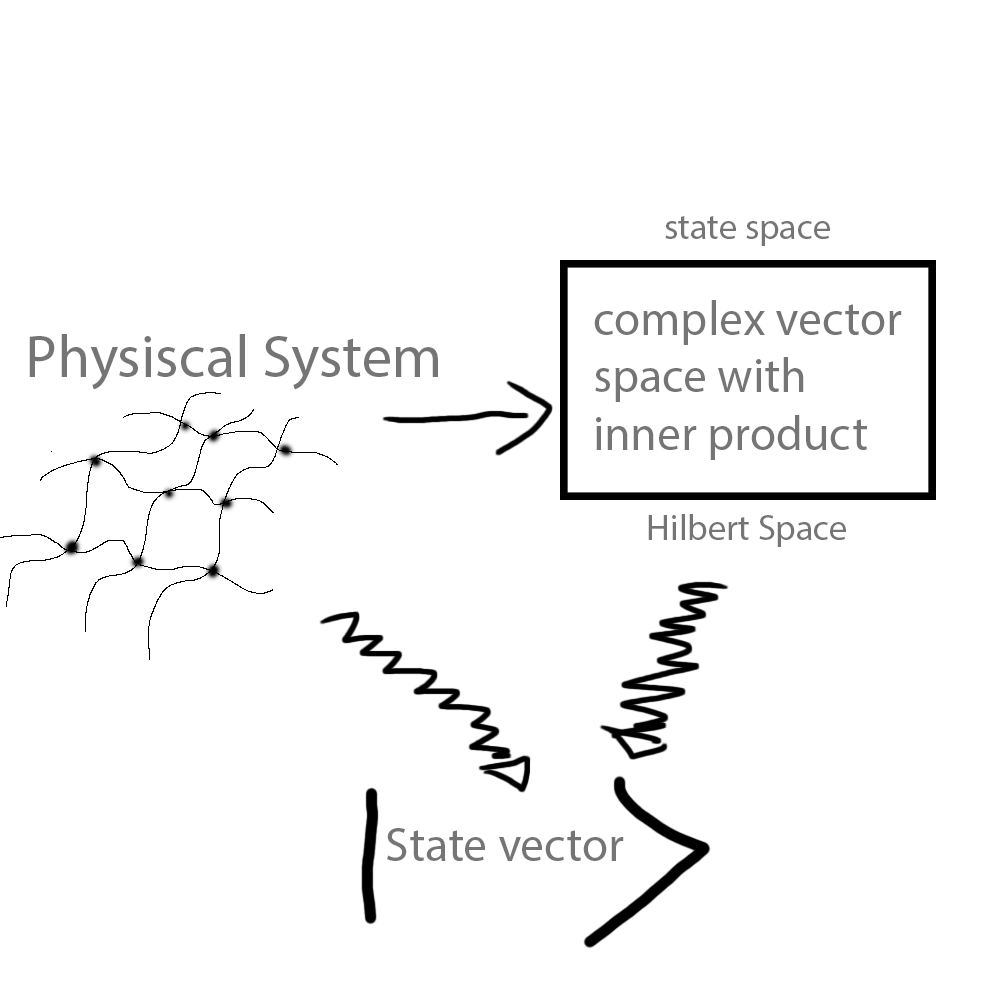
\includegraphics[scale=0.2]{images/sketch1.png} 
%		\caption{how a physical state is represented}
%	\end{figure}
	Every pure quantum state can be represented as vector in a vector space with inner product, i.e. a \emph{Hilbert space}. 
	 A complex Hilbert space $\H$ of dimension $n$ is isomorphic to $ \mathbb{C}^n $ with the standard inner product. 
	 In $\mathbb{C}^n $ one can choose a basis and then represent vectors with coordinates with respect to this basis.
	The bra-ket notation is a handy notation introduced by physicist Paul Dirac to deal with such vector representation of quantum states. 
	First of all we note that a state $\varphi '\in\H$ corresponds via the isomorphism to $ \varphi  \in \mathbb{C}^n $. It can be represented as a vector with respect of some basis as follows
	$$\ket{\varphi} = \begin{pmatrix} \varphi_1 \\ \varphi_2 \\ \vdots \end{pmatrix}	  \text{  is a coloumn "ket" vector over } \H $$
	$$\bra{\varphi}  = \begin{pmatrix} \varphi_1 & \varphi_2 & \hdots \end{pmatrix} \text{  is a row "bra" vector over } \H $$
	To be representative of a quantum state the vector has to have unitary length, $\|\varphi\|= 1$.
	Furthermore the conjugate transpose of a \emph{bra} vector is the corresponding \emph{ket} vector, and vice versa.
	$$ \bra{\varphi}^{\dagger} = \ket{\varphi} \text{,    } \ket{\varphi}^{\dagger} = \bra{\varphi}$$
	More specifically, for a complex vector space as $\H$, the components of $\bra{\varphi}$ are each the complex conjugate of the components of $\ket{\varphi}$.
	It is worth noting that in quantum information we will consider only vectors of finite dimensions, and more often than not, the standard basis for qubits represented by
	$$\ket0 =  \begin{pmatrix} 1 \\ 0 \end{pmatrix}
	\text{ and }
	\ket1 =  \begin{pmatrix} 0 \\ 1 \end{pmatrix}$$
	which are recognizable as the equivalent of $\vec{e_1}$ and $\vec{e_2}$ in $\mathbb{C}^2$.
	
	To summarize then, $\ket{\varphi}$ represents a column vector on a complex vector space with inner product equivalent to $\mathbb{C}^n$ in some basis, and $\bra{\varphi}$ is its complex conjugate.
	
	
	So if we define the matrix\footnote{The fact that the result of  $ \ketbra{w}{v} $ is indeed a matrix can be seen more directly if we remember that this is nothing less than a column-row vectors multiplication.} $A =  \ketbra{w}{v} $ we observe that
	$$ \ket{w}\braket{v}{v'} = \braket{v}{v'}\ket{w} $$	
	which is a convenient way of visualizing the action of matrix $A$. In particular if we divide it like $(\ketbra{w}{v}) (\ket{v'}) $ it is easy to interpret it as \textit{matrix $A$ acting on vector $\ket{v'}$}. The other equivalent form $(\braket{v}{v'})(\ket{w})$ can also be seen as multiplying vector $\ket{w}$ by a value $\braket{v}{v'}$.
	%this part may be too similar to book, page 67...
	
	The intuition of this is that $\ketbra{w}{v}$ can indeed be defined as a (linear) operator from the vector space of $\ket{v}$ to the vector space of $\ket{w}$. 

\section{Measurements on a  basis} \label{measurements}

	To get any information out of a state one has to \textit{measure} it. 
	Measurement is, mathematically, a projection onto some chosen computational basis. 
	The result for each base vector projection is then interpreted as a \emph{probability}. 
	The state then changes after measurement, meaning for example that it will not retain its value as superposition any more.\\

	If Alice has the state $\ket{\psi_i}$ out of $i=1..n$ and all states are orthonormal, then Bob can --- measuring with the same basis --- find out what the choice of $i$ was.
	If the states are not orthonormal there is no quantum measurement capable of distinguishing the states. 
	If the states $\ket{\psi_1}$ and $\ket{\psi_2}$ are not orthogonal, then $\ket{\psi_2}$ has a component orthogonal to $\ket{\psi_1}$, and also a component parallel to it.
	This will lead to a non-zero probability of measuring a value on $\ket{\psi_1}$ for the state $\ket{\psi_2}$.

	\begin{xmpl}\cite{NC10}
		\begin{equation*} 
			Z = \begin{bmatrix} 1 & 0 \\ 0 & -1 \end{bmatrix} \quad P_{+1} = \proj{0} , \; P_{-1} = \proj{1}
		\end{equation*}
		Measurement on qubit $ \ket{\psi} = \frac{\ket0 + \ket1}{\sqrt{2}} $ has probability $p_{+1} = \bra{\psi}P_{+1}\ket{\psi} = \bk{\psi}{0}\bk{0}{\psi} = \frac{1}{2}$ and similarly $p_{-1} = \frac{1}{2}$
			
	\end{xmpl}
    
	\subsubsection*{Linear operators}
	A linear operator between two vector spaces is defined as 
	$$ \mathbf{A}: V\longrightarrow W \text{  ,  }\ket{v_i}\mapsto A\ket{v_i}$$
	$$ \text{ linear in all inputs, i.e.  }  A\left( \sum_i a_i\ket{v_i}\right) = \sum_i a_i A\ket{v_i} \text{  for all } i $$ 
	Looking back at the definition of the matrix $ A = \ketbra{w}{v}$ we can now refer to it as a linear operator from now on.
	Some well-known linear operators acting on single qubits that we will use later on are the \textit{Pauli Matrices}
	$$ I = \begin{bmatrix} 1 & 0 \\ 0 & 1 \end{bmatrix}	 \quad   X = \begin{bmatrix} 0 & 1 \\ 1 & 0 \end{bmatrix}$$
	$$ Y= \begin{bmatrix} 0 & -i \\ i & 0 \end{bmatrix}	 \quad   Z = \begin{bmatrix} 1 & 0 \\ 0 & -1 \end{bmatrix}$$
	
	In particular it is safe to say that, unless stated otherwise, the operators that will be presented all have a set of properties and are called Hermitian operators, or \emph{self-adjoint operators}.
	$$ A = A^{\dagger} \quad \Longrightarrow (A\ket{v})^{\dagger} = \bra{v}A^{\dagger} $$ 
	Operators have also to be positive, this means that it holds, for every $\ket{v}$, $\bra{v}A\ket{v}$ is real non-negative. 
 
\section{Mixed states}
	All pure states in QM are normalized vectors in $\H$.
	$$ \ket{\psi} \text{ is a state vector } \Rightarrow \ket{\psi}\in\H \text{ and }  \vert\bk{\psi}{\psi}\vert = 1$$
	This is instrumental in seeing them as probability vectors. 
	Every linear operator has then to be unitary to maintain this property.
	A statistical mixture of states corresponds to a \emph{density matrix}, which is itself a new state. 
	It is important to note that a mixture of probability of states is not the same thing as superposition of states. In the latter we don't have a measure of uncertainty of the state, meaning also that in theory we are always able to find a measurement basis that will always output the same result for that state. 
	In the former, however, this is not possible because of the intrinsic uncertainty of the state.
	Density matrices have then the properties:
	$$ M = \rho = \sum_i p_i \ketbra{\psi_i}{\psi_i} = \sum_i p_i P_{\ket{\psi_i}} \text{  , where state }\ket{\psi_i}\text{ has probability } p_i $$ 
	$\rho$ is a positive, trace-1 operator meaning that $\Tr(\rho) = 1$ and all eigenvalues of $\rho$ are positive. 
	Moreover $\rho$ is a linear combination of projectors $\proj{\psi_i}$ which makes $\rho\in\mathbb{P}(\H)$ a projector itself on the the Hilbert space.

%\section{Quantum entanglement}
%
%	\begin{quotation}
%		There exist vectors in $V\otimes W$ that can not be represented by a single tensor product:
%		Given $v_1,v_2\in V \; w_1,w_2\in W$ linear independent:
%    \begin{equation*}
%		v_1\otimes w_1 + v_2\otimes w_2 = v_1w_1 + v_2w_2 \in V\otimes W
%    \end{equation*}
%    is \emph{not} separable.
%		this may be strange because on physical level tensor product is combination(merging) of quantum systems
%		\end{quotation}\cite{Han13}